\section{SSAA 的四个着色样点}

Sponza 中庭的场景面板输出 $384\times246$ 个像素。打开「SSAA 2×2」后，模型表面、光照和屏幕效果先画成 $768\times492$；同一块面板像素对应四个内部位置。图中两次运行均取编辑器第 24 帧。镜头、灯光和曝光设置相同，右侧树叶与石地的局部按同一倍率放大。

\begin{figure}[H]\centering
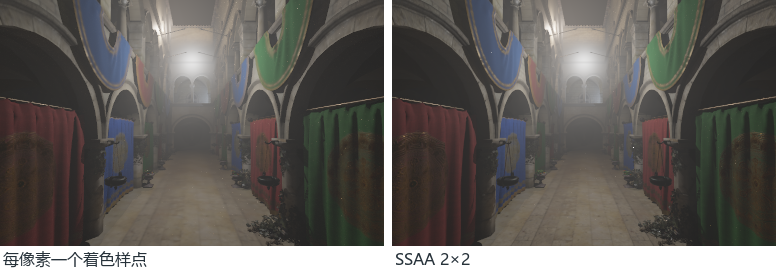
\includegraphics[width=.96\linewidth]{ssaa/sponza.png}\par\vspace{5pt}
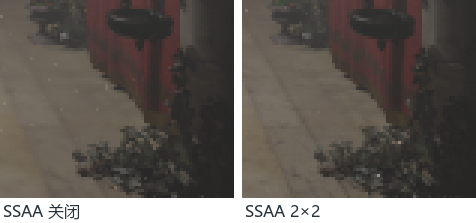
\includegraphics[width=.64\linewidth]{ssaa/foliage.png}
\caption{上图来自 Vulkan 编辑器最终送往场景面板的颜色图。下图取原图从 $(222,173)$ 开始的 $78\times66$ 像素，放大三倍。房间内的 TAA、DDGI、GTAO、反射和雾均参与这次绘制。}
\end{figure}

\ssaaExample\par

\ssaaVerified\par

同一机位另用前一版程序画了一次。无论关闭还是开启 SSAA，两版输出的 8 位颜色图均逐像素相同。要观察新算法怎样保留远处的细线，可以看相机移过斜纹时的连续帧。\par

\readings{\href{run:../profiling/ssaa/on-replay.json}{四个样点与逐像素核验}\quad
\href{run:../profiling/ssaa/off-replay.json}{关闭时的回放}\quad
\href{run:../profiling/ssaa/sponza.png}{完整画面}\quad
\href{run:../validation/mask-footprint-compare-rank/diagonal-motion.png}{移动相机经过斜纹}}

\newpage
\section{Sponza 的显存与耗时}

这次使用 Debug x64 编辑器（\texttt{\ssaaBuild}）和 RTX 5070 Ti Laptop GPU。实际编辑视口为 $1391\times892$，场景面板的输出宽度固定为 384。103 次绘制写入供光照读取的模型表面，另有 103 次供编辑器拾取、22 次画界面。开关 SSAA 的绘制次数相同，打开后，光照和屏幕效果需要处理四倍的内部像素。

{\smalltable\noindent\begin{tabularx}{\linewidth}{@{}Xrr@{}}\toprule
渲染资源 & 关闭 & SSAA 2×2\\\midrule
\ssaaStorage
\bottomrule\end{tabularx}\par}

缓冲区取 RenderDoc 在捕获中列出的长度，图像取纹理条目的字节数。两帧都登记了 232 个缓冲区和 319 张图像，合计多出约 75 MiB，其中约 65 MiB 来自缓冲区。这个差值反映两份截帧列出的资源大小；要测驱动实际驻留的显存峰值，还需跟踪分配与释放。

{\smalltable\noindent\begin{tabularx}{\linewidth}{@{}Xrr@{}}\toprule
测量范围（毫秒） & 关闭 & SSAA 2×2\\\midrule
\ssaaTimes
\bottomrule\end{tabularx}\par}

GPU 时间来自 RenderDoc 1.47 的事件计数器。按关、开、开、关回放，每轮先预热一次，再取六次；将同组事件在一次回放内相加，再取该设置 12 次结果的中位数。绘制与计算的合计覆盖列出的事件，帧中另有清屏、复制、等待与呈现。提交队列的数字是截帧当次主机调用 \code{vkQueueSubmit} 的用时之和，各一帧。

整帧数据来自未挂 RenderDoc 和 Vulkan 验证层的六次独立启动。每种设置先后启动三次。面板最后一次调整大小后，每次跳过前八帧，记录 24 帧重画，另记录 16 帧沿用已有面板图。整帧计时包括主线程等待 GPU 和窗口呈现。P95 表示约 95\% 的样本用时低于该值。两种设置的计算派发相差约 17 毫秒。若要缩短本场景的重画时间，可先分别测量反射与雾在两种分辨率下的用时。\par

\readings{\href{run:../profiling/ssaa/gpu.json}{GPU 每次回放与提交时间}\quad
\href{run:../profiling/ssaa/editor.json}{编辑器逐帧耗时}\quad
\href{run:../profiling/ssaa/on-capture.json}{程序、设置与原始帧校验值}\quad
\href{run:../../tests/profile_ssaa.py}{复现脚本}}
